\documentclass[a4paper, 11pt]{article}

%\usepackage{xltxtra}

\setmainfont[Mapping=tex-text, Numbers={OldStyle}, Ligatures={Common, Rare, Historical}]{Linux Libertine O}

% aptitude install texlive-lang-spanish
\usepackage[catalan]{babel}

\usepackage{amsmath}
\usepackage{makeidx}
\usepackage{amssymb}
\usepackage{amsmath}
\usepackage{url}
\usepackage[backref]{hyperref}
\usepackage{textcomp}
\usepackage{sverb}
\usepackage[format=plain,labelfont=bf,up,textfont=it,up]{caption}
\usepackage[kerning,spacing]{microtype}
\microtypecontext{spacing=nonfrench}
\usepackage{indentfirst}
\usepackage{float}
\usepackage{fancyhdr}
\usepackage{ifdraft}
\usepackage{amsmath}
\usepackage{subfig}
\usepackage{pgf}
\usepackage{tikz}
\usetikzlibrary{arrows,automata}
\usepackage{booktabs}
\usepackage{array}

\ifdraft{
  \newcommand{\pycode}{
    Codi deshabilitat en mode \emph{draft}. Consulta ``capsalera.tex'' \\
  }
}{
  \usepackage{minted}
  \newcommand{\pycode}[1]{
  \paragraph{#1.py}
    \inputminted[linenos, frame=lines, fontsize=\small]{python}{src/#1.py}
  }
}

\ifdraft{
  \usepackage{savetrees}
}{
}


%%%%%%%%%%%%%%%%%

\usepackage{xltxtra}

\setmainfont{Linux Libertine O}
% \setmainfont[Mapping=tex-text, Numbers={OldStyle}, Ligatures={Common, Rare, Historical}]{Linux Libertine O}

\usepackage[catalan]{babel}
\usepackage{booktabs}
\usepackage{indentfirst}
\usepackage{url}
\usepackage[backref]{hyperref}

%%%%%%%%%%%%%%%%%%

\title{Simulador d'un sistema interactiu}

\author{
  Pau Ruŀlan Ferragut \small{<paurullan@gmail.com>}
}

\date{
\begin{flushright}
  Pràctica de simulació \\
  Convocatòria setembre \\
  Curs 2010--11
\end{flushright}
}

\begin{document}

\maketitle

\thispagestyle{empty}

\abstract{Com exercici pràctica hem construit un simulador d'esdeveniments
  discrets que modela un sistema informàtic interactiu. Un cop implementat el
  simulador l'usarem per determinar el temps de resposta del sistema i estudiar
  el seu comportament a mida que aumentam els usuaris.}

\section{Especificació del problema}

Cal especificar el nostre simulador tant a nivell numèric com en termes de
distribucions estadístiques.

\subsection{Paràmetres d'entrada}

\begin{tabular}{lr}
Paràmetre d'entrada & selecció \\
\toprule
Temps mig de reflexió  & 10 seg \\
Nombre d'usuaris & variable $X$ \\
Velocitat de CPU & 2500 pps \\
Velocitat de disc & 15.000 rpm \\
Peticions de disc per transacció & 5 peticions \\
Temps de resposta del sistema & variable $Y$ \\
Throughput & no \\
Utilització CPU & no \\
Utilització disc & no \\ 
\end{tabular}

\subsection{Modelització dels components}

El nostre simulador està caracteritzat per tres components: la població, la CPU
i el disc dur.

\subsubsection{La població}

Els distints usuaris entren al sistema fent una petició i, un cop resolta,
s'esperen un temps de reflexió.

\paragraph{Distribució de la població}

La població es pot modelar mitjançant una distribució exponencial de mitja 10
segons, $Exp(10)$.

\subsubsection{La CPU}

S'ha escollit un processador comercial AMD Opteron 6140, de capacitat de
treball de 62,4K MIPS\cite{cpu_specs}. Aquest valor és pel conjunt dels vuit
nuclis però podem limitar la simulació a un sol nucli, donant aproximadament
uns 7,5K MIPS. Suposam que una visita són 3M instruccions de promig. La
capacitat de servei i el temps de servei mig són:

\[ \mu = 7,5K MIPS \times \frac{1\text{M instruccions}}{1 \text{seg}} 
                \times \frac{1 \text{transacció}}{3 \text{M instruccions}} \]

\[ \mu = 7,5K MIPS \times \frac{1{M instruccions}}{1 {seg}} 
                \times \frac{1 {transacció}}{3 {M instruccions}} \]

\[ \mu = 2.500 \, \frac{transaccions}{s}\]

\[ s = \frac{1}{\mu} = 0,4 \, ms \]

\paragraph{Distribució de la CPU}

La CPU queda modelada amb una distribució constant $C(0,4)$, en ms.

\subsubsection{El disc dur}

S'ha usat un disc dur de servidor model Seagate Cheetah
15K\cite{disc_specs}. Els discs durs clàssics es composen de tres tasques
seqüencials: búsqueda (\emph{seek}), latència i transfarència. Aquestes tasques
es modelen típicament mitjançant distribucions exponencials, uniformes i
constants respectivament.

Aquest disc dur està especificat com:

\begin{itemize}

  \item Velocitat de rotació 15.000 rpm

  \item Temps de seek del fabricant 3,4 ms

  \item Temps de latència del fabriant 2 ms

  \item Velocitat de transfarència 600 MB/s

\end{itemize}

Suposam un conjunt de fitxers grans, com documents PDF, de tamany 1,5MB. Aquest
fitxers també els suposarem dispersats aleatòriament al llarg del disc però amb
els seus blocs continuus. És a dir, obtenir un fitxer consistirà en:

\[ T = seek + lat + trans \]

\paragraph{Càlcul del \emph{seek}}

Com que al nostre exercici sols feim lectures podem usar el temps de
\emph{seek} mig de lectura especificat pel fabricant de 3,4 ms. Aquest
estadístic es comporta com una distribució exponencial $Exp(3,4)$ en ms.

\paragraph{Càlcul de la latència}

El nostre disc té una velocitat de rotació de 15.000 rpm, per la qual cosa
presenta un temps de volta de 4 ms. Això implica una distribució uniforme $U(0,
4)$ en ms. Cal fixar-se que el fabricant ja havia indicat que la latència mitja
era de 2ms.

\[ 15.000 \text{rpm} \, \frac{1 \text{ min}}{60 \text{ seg}} = 250 \text{rps}
= 4 \text{ ms}\]


\paragraph{Càlcul de la transfarència}

El temps de transfarència ve pel temps de rotació sobre un sector. El fabricant
ens especifica que són 600 MB/s i donat que el nostre fitxer és de 1,5MB tardam
2,5ms de transfarència. Això implica una distribució constant de $C(2,5)$ en
ms.

\[ 600 \, \text{MB} \, \frac{1 \text{ tasca}}{1,5 \text{ MB}}
       = 400 \text{ tasques} = 2,5 \text{ ms}\]

\paragraph{Distribució del disc dur}

D'aquesta manera el disc dur es pot modelar mitjançant una distribució composta
per la del \emph{seek}, la latència i la transfarència juntament amb la forma
del nostre fitxer (en ms):

\[ Exp(3,4) + U(0, 4) + C(2,5) \]

%\section{El simulador}

Anam a definir com està organitzat el nostre simulador.

\paragraph{Esdeveniments}

\begin{enumerate}

  \item Tasca d'usuari: un usuari ha acabat de reflexionar i llança una tasca
    cap a la CPU.

  \item Sortida de la CPU: una transacció surt de la CPU i pot anar al disc o
    tornar a reflexionar. Aquesta decisió està codificada estadísticament
    segons el nombre de peticions a disc per transacció.

  \item Sortida del disc: una transacció del disc sempre passa per la CPU.

\end{enumerate}

\paragraph{Variables d'estat}

\begin{enumerate}

  \item Rellotge global

  \item Instant de sortida d'una tasca

  \item Instant d'arribada d'una tasca

\end{enumerate}

\paragraph{Variables estadístiques}

\begin{enumerate}

  \item Temps de processament acumulat, necessari per calcular els temps de
    processament mig.

  \item Nombre de repeticions totals.

\end{enumerate}

\subsection{Organització interna}

El simulador consta de varis mòduls:

\begin{description}

  \item[Principal] coordinador entre els distints mòduls. Està programat al
    fitxer \verb+main.py+ i \verb+sim.py+.

  \item[Inicialitzador] posa a zero els valors i omple de tasques els servidors
    dels usuaris. Està adins el \verb+sim.py+.

  \item[Temporització] mitjançant una cua de prioritats gestiona els distints
    esdeveniments i calcula el següent a llançar. També està a \verb+sim.py+.

  \item[Esdeveniments] genera la resposta a un esdeveniment escollit per la
    temporització. Es troba dins el model de cada servidor, a \verb+model.py+.

  \item[Aleatoris] ampliació del mòdul escrit a PL1 per cobrir les
    distribucions contants i exponencials, al \verb+rand.py+.

  \item[Informe] ajuda a determinar el final de la simulació. També genera els
    càlculs estadístics i les gràfiques. Són els mòduls \verb+statistic.py+,
    \verb+suite.py+ i \verb+chart_generation.py+.

\end{description}

El diagrama de blocs es troba generalitzat al gràfic
~\ref{sim:fig:diagrama-moduls}.

\begin{figure}
  \centering
  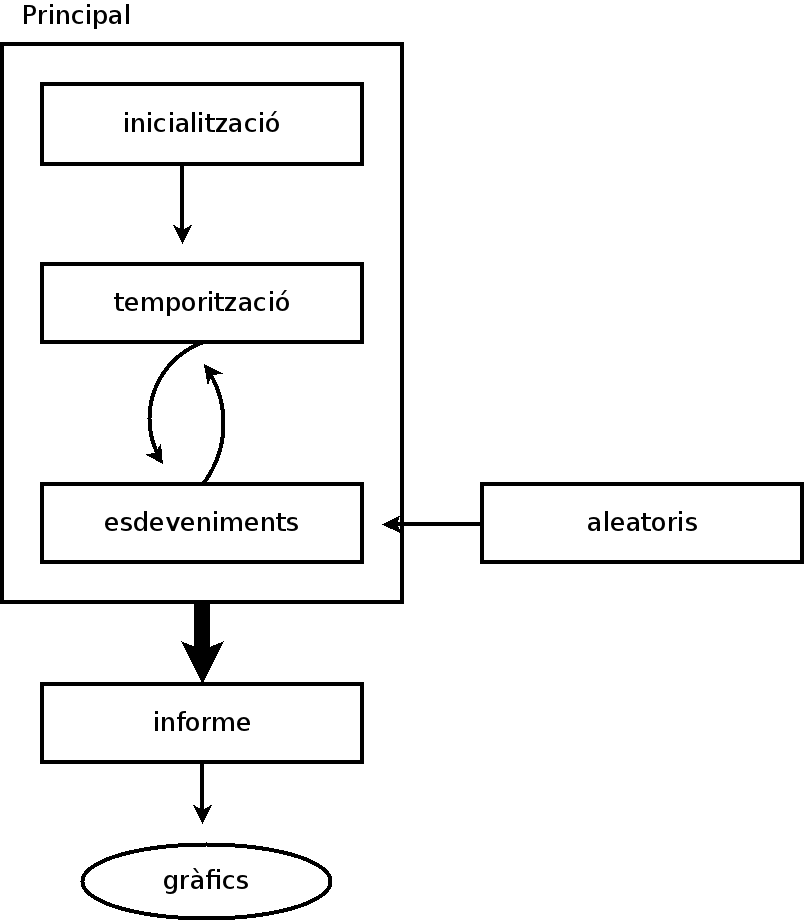
\includegraphics[width=\textwidth]{img/diagrama-moduls.png}
  \caption{Diagrama de mòduls del simulador.}
  \label{sim:fig:diagrama-moduls}
\end{figure}

\section{Pseudocodi}

El pseudocodi del simulador el podem trobar a la figura
~\ref{sim:codi:pseudocodi}.

\begin{figure}
  \centering
  \pycode{pseudocodi}
  \caption{Pseudocodi general del simulador.}
  \label{sim:codi:pseudocodi}
\end{figure}


\section{Desenvolupament}

Sobre el desenvolupament real del simulador cal dir:

\begin{enumerate}

  \item S'ha programat amb el llenguatge de propòsit general Python.

  \item No s'ha duit a terme la validació amb QNAP2.

  \item Per determinar el tamany del transitori s'han fet distintes proves amb
    la durada de la simulació. Llavors hem tallat considerant la primera meitat
    dels esdeveniments transitori.

  \item S'han fet un mínim de 50 rèpliques per variable de nombre de clients i
    llavors se n'han fet tantes com ha calgut per obtenir una desviació de
    manco el 0,1.

\end{enumerate}

%\section{Resultats}

\subsection{Determinació del transitori}

El procés de càlcul del transitori és un poc bast però efectiu: calculàrem
distintes traces per un nombre de clients suficientment gran (100, 200, 250 i
300) i estudiàrem a partir de quin punt el sistema es comportava de manera
estable o cíclica. Com a regla general vàrem poder apreciar que obtenint uns
vint esdeveniments per client i quedant-nos sols amb la segona meitat de tota
la simulació els resultats eren estables.

A les gràfiques es mostra la tendència dels temps de resposta al llarg d'una
simulació.

\newcommand{\grafictransitori}[2]{
\begin{figure}[t]
  \centering
  \includegraphics[width=\textwidth]{img/evo-#1.png}
  \caption{Execució amb #1 clients per estudiar el transitori}
  \includegraphics[width=\textwidth]{img/evo-#2.png}
  \caption{Execució amb #2 clients per estudiar el transitori}
\end{figure}
}

\grafictransitori{100}{200}
\grafictransitori{250}{300}

\subsection{Càlcul de temps de resposta}

Per determinar el punt d'inflexió del nostre sistema calcularem els distints
temps de resposta a mida que anam aumentant els clients. Els temps de resposta
de les simulació es poden llegir a la figura ~\ref{resultats:temps:taula} i es
poden veure representats en la gràfica ~\ref{resultats:temps:grafica}.


\begin{figure}
\centering
\begin{tabular}{lrlr}
N usuaris & TR (ms) &
N usuaris & TR (ms) \\

\toprule

10    & 42.08    &  
260   & 1573.98  \\ 
20    & 42.26    &  
270   & 1961.58  \\
30    & 44.75    &  
280   & 2334.91  \\ 
40    & 49.49    &  
290   & 2688.70  \\
50    & 56.00    &  
300   & 3060.17  \\ \midrule
60    & 56.66    &  
310   & 3421.07  \\
70    & 63.94    &  
320   & 3809.61  \\  
80    & 63.48    &  
330   & 4203.65  \\ 
90    & 66.70    &  
340   & 4591.56  \\ 
100   & 75.61    &  
350   & 4983.98  \\ \midrule
110   & 73.92    &  
360   & 5382.18  \\ 
120   & 87.58    &  
370   & 5762.88  \\
130   & 84.71    &  
380   & 6181.55  \\ 
140   & 91.32    &  
390   & 6584.32  \\
150   & 110.19    &  
400   & 6949.67  \\ \midrule
160   & 110.71    &  
410   & 7346.90  \\
170   & 120.57    &  
420   & 7755.98  \\ 
180   & 137.82    &  
430   & 8086.00  \\
190   & 190.46    &  
440   & 8511.05  \\ 
200   & 254.08    &  
450   & 8891.28  \\ \midrule
210   & 356.87    &  
460   & 9328.79  \\ 
220   & 484.69    &  
470   & 9732.96  \\
230   & 624.87    &  
480   & 10146.00  \\ 
240   & 748.87    &  & \\
250   & 1198.98  &  & \\ 

\bottomrule

\end{tabular}
  \caption{Evolució dels temps de resposta segons es van afegint
    usuaris. Aquestes simulacions són de rèpliques.}

  \label{resultats:temps:taula}

\end{figure}


\begin{figure}
  \centering
  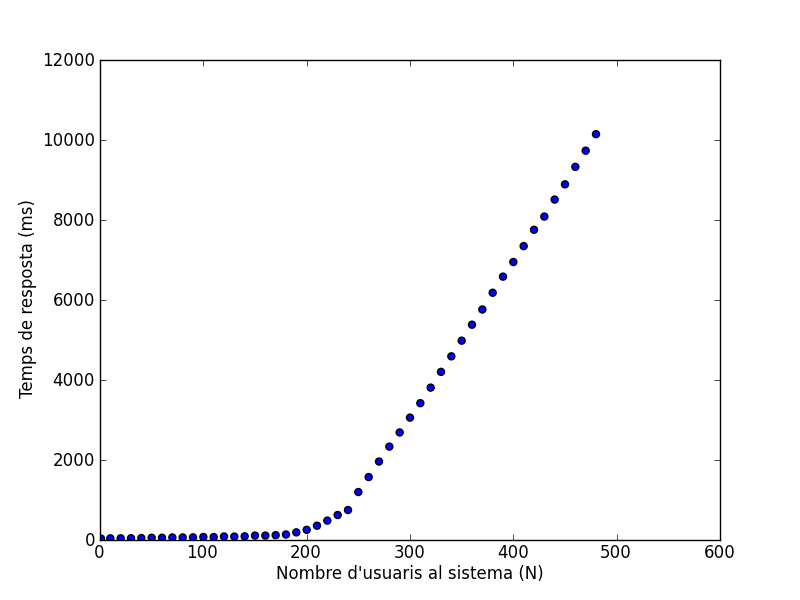
\includegraphics[width=\textwidth]{img/sim.png}

  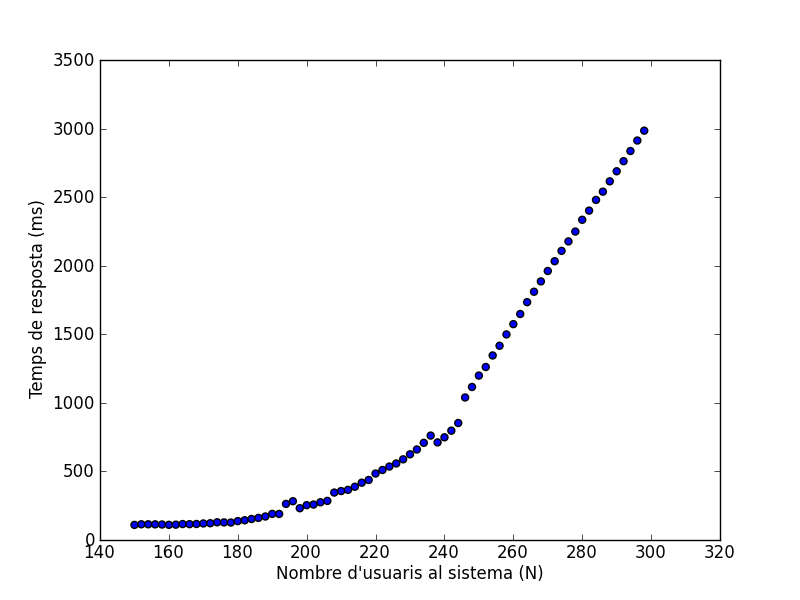
\includegraphics[width=\textwidth]{img/sim-retall-150-300.png}

  \caption{Evolució dels temps de resposta segons es van afegint usuaris en
    simulacions mitjançant rèpliques.}
  \label{resultats:temps:grafica}

\end{figure}

Després de les simulacions podem observar i concloure que:

\begin{enumerate}

  \item Sols hem utilitzat un processador pel nostre servidor, de temps de
    servei $0.4ms$.

  \item El disc té un temps de servei de casi $8ms$.

  \item Una operació demana una mitja de cinc transaccions de disc.

  \item Fins als 200 usuaris el sistema manté un temps de resposta d'un quart
    de segon ($250ms$), rendiment acceptable per una aplicació interactiva.

  \item A partir dels 250 usuaris l'aplicació passa a tenir un temps de
    resposta d'un segon, fent-la adient sols per aplicacions no purament
    interactives.

  \item Des dels 200 usuaris, afegint un 0.25 de càrrega hem quadruplicat el
    temps de resposta. Podem afirmar que entre el rang de 200 i 250 usuaris
    tenim el punt d'inflexió del sistema.

  \item Malgrat no tinguem els càlculs de l'utilització de la CPU, la
    diferència de magnitud de temps de resposta amb el disc (vint vegades) ens
    indica que probablement el coll de botealla és el disc.

\end{enumerate}

\paragraph{Conclusions}

Recordant que hem modelat un sistema amb un processador i un disc modern i
potent podem veure el gran nombre d'usuaris que s'han de menester per saturar
el sistema. El coll de botella és el disc dur doncs és casi vint vegades més
lent que el processador. De tota manera cal recordar que si consideràssim un
temps de resposta inacceptable a partir del segon ja estam parlant de casi 250
usuaris concurrents per un conjunt \emph{hardware} que no arriba ni als 1000€.

D'aquesta manera i malgrat hem fet grans simplifiacions, com obviar que els
computadors actuals estan provistos d'un important conjunt de memòries cau, hem
pogut valorar quantitativament el rendiment del sistema i jugar amb el que
podria ser la implementació d'un sistema de simulació.

\begin{thebibliography}{9}

\bibitem{cpu_specs} AMD Opteron 6140

\url{http://www.amd.com/es/products/server/processors/6000-series-platform/pages/6000-series-platform.aspx} \\

\url{http://www.cisco.com/web/DK/assets/docs/presentations/vBootcamp_Performance_Benchmark.pdf}

\bibitem{disc_specs} Seagate Cheetah 15K

\url{http://www.seagate.com/www/en-us/products/enterprise-hard-drives/cheetah-15k#tTabContentSpecifications}

\end{thebibliography}


\newpage

\appendix

%\newpage

\addtolength{\hoffset}{-2cm}

\section{Codi font}

En aquest apèndix trobarem el codi de l'aplicació, el petit programa per
obtenir les gràfiques del transitori i els jocs de prova.

\subsection{Codi general}

Aquí trobarem els distints fitxers del la nostra pràctica:

\begin{description}

  \item[main.py] Programa principal.

  \item[suite.py] Gestor de tasques i llançament de rèpliques.

  \item[sim.py] El mòdul principal de la simulació.

  \item[model.py] Modelització dels usuaris, la cpu i el disc.

  \item[rand.py] El nostre mòdul de nombres aleatoris.

  \item[statistic.py] Mòdul del càlcul estadístic.

  \item[chart\_generator.py] Mòdul per pintar les gràfiques.

\end{description}

\pycode{main}
\pycode{suite}
\pycode{sim}
\pycode{model}

\pycode{rand}
\pycode{statistic}
\pycode{chart-generator}

\newpage

\subsection{Càlcul del transitori}

Hem usat aquest petit programa per obtenir un parell de mostres gràfiques i
així tenir pistes sobre com determinar el transitori.

\pycode{calcul-transitori}

\newpage

\subsection{Jocs de prova}

Per la tasca de programació hem aprofitat per aplicar per primera vegada un
model de programació anomenat \emph{programació dirigida per proves} (de
l'anglès \emph{test driven development} o TDD). El que es fa és \emph{primer}
escriure els jocs de proves per cadasqun dels mètodes que es van necessitant i
no s'avança a la següent característica fins que totes les proves anteriors
funcionen. Aquesta metodologia pot pareixer més engorrosa però un cop el
programa va més enllà d'un petit mòdul i alguna gràfica s'accelera la
programació per que és molt senzill detectar els problemes causats pel nou
desenvolupament.

Aquest comentari el feim per indicar que el gran nombre de tests de a causa de
l'estil de programació poc habitual.

\pycode{test-chart}
\pycode{test-rand}
\pycode{test-statistic}
\pycode{test-model}
\pycode{test-sim}
\pycode{test-sim-queue}
\pycode{test-suite}

\newpage

\addtolength{\hoffset}{+2cm}


\end{document}
